\section{Schwachstelle 6: Local-Privilege-Escalation bei win.int.mb-reps.cool.datcom.prv}
\label{sec:vuln6}
Über den in Kapitel \ref{sec:vuln5} vorgestellten Weg zur Kompromittierung des \texttt{win}-Hosts konnte weiterführend eine Local-Privilege-Escalation aufgrund der Gruppenmitgliedschaft \texttt{lxd} ausgentuzt und somit Root-Berechtigungen erlangt werden. 

\subsection{Beschreibung der Schwachstelle}
\label{subsec:vuln6_way}
Der Angriff gliedert sich in zwei Teile und ist im Detail unter \url{https://www.exploit-db.com/exploits/46978} beschrieben. Zuerst wird auf der Angreifer-Maschine ein LXC-Container-Image erstellt, das anschließend mit der bereits bestehenden Meterpreter-Session zur \texttt{win}-Maschine heruntergeladen wird. Im zweiten Teil des Angriffs wird eine Instanz des hochgeladenen Container-Images erstellt und das Dateisystem des \texttt{win}-Hosts innerhalb des LXC-Containers gemountet. Anschließend kann der Angreifer sich zur Instanz des LXC-Containers verbinden und mit Root-Berechtigungen innerhalb des gemounteten Dateisystems beliebige Lese- und Schreib-Operationen durchführen, welche sich somit auch auf das Dateisystem des \texttt{win}-Hosts wiederspiegeln. Es wird gezeigt, wie das \texttt{setuid}-Bit für \texttt{/bin/bash} gesetzt und dadurch Root-Berechtigungen erlangt werden können.

Auflistung \ref{lst:vuln6_searchsploit} zeigt, wie mittels der Suche über \texttt{searchsploit} die Schwachstelle und das dazugehörige Shell-Skript gefunden wurde.

\lstset{language=bash,caption={Suche nach Schwachstellen in Ubuntu 18.04 über \texttt{searchsploit}}, label=lst:vuln6_searchsploit}
\begin{lstlisting}[frame=single, firstnumber=1, stepnumber=1,]
|--(gu4c4m0l3@kali-t470)-[~]
|-$ searchsploit Ubuntu 18.04
------------------------------------------ ------------------------
 Exploit Title                            |  Path
------------------------------------------ ------------------------
Ubuntu 18.04 - 'lxd' Privilege Escalation | linux/local/46978.sh
------------------------------------------ ------------------------
Shellcodes: No Results
\end{lstlisting} 

\subsubsection{Erstellen des LXC-Imagess auf der Kali-VM}
Zuerst wird das Build-Skript zum bauen des LXC-Images mit dem Befehl \texttt{wget https://raw.githubusercontent.com/\-saghul/\-lxd-alpine-builder/\-master/build-alpine} heruntergeladen und anschließend als ausführbar markiert (\texttt{chmod +x build-alpine}). Danach kann mit starten des Build-Skripts die LXC-Imagedatei erstellt werden. Befehl: \texttt{./build-alpine}. Es wurde eine neue Image-Datei im gleichen Ordner mit dem Namen \texttt{alpine-v3.15-x86\_64-20220301\_1532.tar.gz} erstellt. 

\subsubsection{Hochladen und Ausführen des LXC-Images}
Anschließend wurde die LXC-Image-Datei in den \texttt{/tmp}-Ordner des \texttt{win}-Rechners über die bereits bestehende Meterpreter-Sitzung hochgeladen (s. Textauszug \ref{lst:vuln6_upload_lxc_image}).

Darüber hinaus wurde das über \texttt{searchsploit} gefundene Shell-Skript ebenfalls hochgeladen.

\lstset{language=bash,caption={Upload der Exploit-Dateien zum \texttt{win}-Host}, label=lst:vuln6_upload_lxc_image}
\begin{lstlisting}[frame=single, firstnumber=1, stepnumber=1,]
meterpreter > upload Documents/pentest_MB-Reps/172_16_34_42/alpine-v3.15-x86_64-20220301_1532.tar.gz /tmp/image
[*] uploading  : /home/gu4c4m0l3/Documents/pentest_MB-Reps/172_16_34_42/alpine-v3.15-x86_64-20220301_1532.tar.gz -> /tmp/image
[*] Uploaded -1.00 B of 3.09 MiB (0.0%): /home/gu4c4m0l3/Documents/pentest_MB-Reps/172_16_34_42/alpine-v3.15-x86_64-20220301_1532.tar.gz -> /tmp/image
[*] uploaded   : /home/gu4c4m0l3/Documents/pentest_MB-Reps/172_16_34_42/alpine-v3.15-x86_64-20220301_1532.tar.gz -> /tmp/image

meterpreter > upload /usr/share/exploitdb/exploits/linux/local/46978.sh /tmp/
[*] uploading  : /usr/share/exploitdb/exploits/linux/local/46978.sh -> /tmp/
[*] uploaded   : /usr/share/exploitdb/exploits/linux/local/46978.sh -> /tmp//46978.sh
\end{lstlisting} 


Anschließend wurde das Shell-Skript \texttt{/tmp/46978.sh} als ausführbar markiert und mit Angabe der Image-Datei im \texttt{f}-Parameter ausgeführt (s. Abbildung \ref{fig:vuln6_execute_exploit}).

\begin{figure}[htbp]
    \centering
    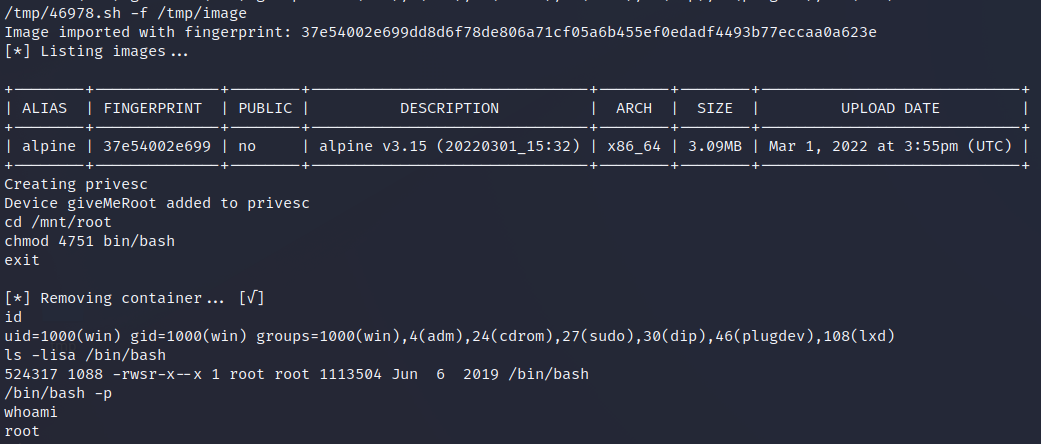
\includegraphics[width=\textwidth]{./img/vuln6_privesc/vuln6_execute_privesc}
    \caption{Ausführen des Privilege-Escalation-Exploits auf dem \texttt{win}-Host.}
    \label{fig:vuln6_execute_exploit}
\end{figure}

Die damit erhaltene Kommandozeileneingabe wird mit den Root-Berechtigungen des LXC-Containers (Achtung: nicht mit den Root-Berechtigungen des \texttt{win}-Hosts) ausgeführt. Über den Mountpunkt \texttt{/mnt/root} kann allerdings nun auf das Dateisystem des \texttt{win}-Hosts mit Root-Berechtigungen gelesen und geschrieben werden. Die Abbildung zeigt, wie dadurch unter \texttt{/mnt/root/bin/bash} bzw. bei dem \texttt{win}-Host unter \texttt{/bin/bash} die Bash-Datei mit dem \texttt{setuid}-Bit (Befehl: \texttt{chmod 4751 bin/bash}) gesetzt wird, sodass bei jeder Ausführung der Bash-Datei diese mit Root-Rechten gestartet wird. Von diesem Zeitpunkt an hat ein Angreifer das System unter voller Kontrolle und kann das Root-Passwort ändern oder neue Benutzer oder Cron-Jobs zum System hinzufügen.

Mit dem Befehl \texttt{exit} kann anschließend der Container verlassen werden und das zuvor ausgeführte Shell-Skript entfernt die entstandenen Container-Dateien. Anschließend kann mit \texttt{/bin/bash -p} eine Bash-Shell mit Root-Rechten gestartet werden. 

Die Passwort-Hashwerte aus der \texttt{/etc/shadow}-Datei konnten anschließend mit gängigen Passwort-Wörterlisten nicht gebrochen werden.

\subsection{Risikobewertung}
Voraussetzung für die Durchführung der Rechte-Eskalation, ist der vorherige Zugriff durch den Command-Shell-Tunnel (s. Schwachstelle 5). Daher wird die Eintrittswahrscheinlichkeit mit NIEDRIG bewertet. Im Falle einer Rechte-Erweiterung erhält ein Angreifer Root-Berechtigungen und hat somit die Kontrolle des Systems übernommen. Daher wird die Schadenshöhe mit HOCH bewertet.

Das Gesamtrisiko wurde daher mit \textcolor{orange}{MITTEL} bewertet.

\subsection{Empfohlene Gegenmaßnahmen}
Es wird empfohlen das Betriebssystem auf die neueste Version zu aktualisieren und die \texttt{lxd}-Gruppenmitgliedschaft beim \texttt{win}-Benutzer zu entfernen, sofern keine geschäftlichen Belange dagegen sprechen.

\subsection{Hinterlassene Spuren und Spurenbeseitigung}
Es wurden im \texttt{/tmp/}-Ordner die Dateien \texttt{image} und \texttt{46978.sh} hochgeladen, welche mit dem Befehl \texttt{rm /tmp/46978.sh /tmp/image} nach dem Pentest über die Verwendung des Command-Tunnels (Port 4444) entfernt wurden.



